% Generated by figures/_scene.py (Scene.render_tikz) for 'Fig 2 stages'; do not edit by hand, re-run the figure script.
% 6.875 x 4.42 in at 100 %; needs \usetikzlibrary{arrows.meta}; images in Figures/fig2/.
{%
\definecolor{c1D221C}{HTML}{1D221C}%
\definecolor{c2A9D8F}{HTML}{2A9D8F}%
\definecolor{c2B3A67}{HTML}{2B3A67}%
\definecolor{c30638E}{HTML}{30638E}%
\definecolor{c4A78B5}{HTML}{4A78B5}%
\definecolor{c5F685C}{HTML}{5F685C}%
\definecolor{c6AA84F}{HTML}{6AA84F}%
\definecolor{c888888}{HTML}{888888}%
\definecolor{c8A8A8A}{HTML}{8A8A8A}%
\definecolor{cB8860B}{HTML}{B8860B}%
\definecolor{cC0392B}{HTML}{C0392B}%
\definecolor{cD9E2F3}{HTML}{D9E2F3}%
\definecolor{cE0A82E}{HTML}{E0A82E}%
\definecolor{cEEF3FA}{HTML}{EEF3FA}%
\definecolor{cF1F8EE}{HTML}{F1F8EE}%
\definecolor{cF4F4F2}{HTML}{F4F4F2}%
\definecolor{cFBE3C4}{HTML}{FBE3C4}%
\definecolor{cFDF8EA}{HTML}{FDF8EA}%
\definecolor{cFFFFFF}{HTML}{FFFFFF}%
\begin{tikzpicture}[x=1in, y=1in]%
\useasboundingbox (0,0) rectangle (6.8750,4.4200);
\draw[draw=cE0A82E, line width=1.200pt, fill=cFDF8EA, rounded corners=0.0900in] (0.4000,2.7200) rectangle (4.9800,4.2800);
\draw[draw=cE0A82E, line width=0.900pt, fill=cFFFFFF, rounded corners=0.0500in] (0.5400,4.1700) rectangle (2.3858,4.3900);
\draw[draw=c6AA84F, line width=1.200pt, fill=cF1F8EE, rounded corners=0.0900in] (0.4000,1.4000) rectangle (4.9800,2.5600);
\draw[draw=c6AA84F, line width=0.900pt, fill=cFFFFFF, rounded corners=0.0500in] (0.5400,2.4500) rectangle (2.6363,2.6700);
\draw[draw=c4A78B5, line width=1.200pt, fill=cEEF3FA, rounded corners=0.0900in] (0.4000,0.0400) rectangle (4.9800,1.2400);
\draw[draw=c4A78B5, line width=0.900pt, fill=cFFFFFF, rounded corners=0.0500in] (0.5400,1.1300) rectangle (2.1352,1.3500);
\draw[draw=c2B3A67, line width=0.900pt, fill=cD9E2F3, line join=round] (2.6200,3.0300) -- (3.2923,3.2292) -- (3.2923,3.6608) -- (2.6200,3.8600) -- cycle;
\draw[draw=c2B3A67, line width=0.900pt, fill=cFBE3C4, line join=round] (3.3273,3.2458) -- (3.9000,3.1130) -- (3.9000,3.7770) -- (3.3273,3.6442) -- cycle;
\draw[draw=c888888, line width=0.900pt, fill=cFFFFFF, rounded corners=0.0500in] (0.5200,1.5500) rectangle (1.7700,2.2700);
\draw[draw=c2B3A67, line width=1.000pt, fill=cFFFFFF, rounded corners=0.0500in] (2.3000,1.5500) rectangle (3.5500,2.2700);
\draw[draw=c2B3A67, line width=0.900pt, fill=cD9E2F3, line join=round] (2.2300,0.4200) -- (2.8591,0.5256) -- (2.8591,0.7544) -- (2.2300,0.8600) -- cycle;
\draw[draw=c2B3A67, line width=0.900pt, fill=cFBE3C4, line join=round] (2.8941,0.5344) -- (3.4300,0.4640) -- (3.4300,0.8160) -- (2.8941,0.7456) -- cycle;
\draw[draw=c8A8A8A, line width=1.300pt, fill=cF4F4F2, rounded corners=0.0900in] (5.1000,0.0400) rectangle (6.8550,4.2800);
\draw[draw=cC0392B, line width=0.600pt, fill=cC0392B, rounded corners=0.0120in] (5.2400,3.6500) rectangle (5.3600,3.7700);
\draw[draw=cC0392B, line width=0.600pt, fill=cFFFFFF, rounded corners=0.0120in] (5.3950,3.6500) rectangle (5.5150,3.7700);
\draw[draw=cC0392B, line width=0.600pt, fill=cC0392B, rounded corners=0.0120in] (5.5500,3.6500) rectangle (5.6700,3.7700);
\draw[draw=cC0392B, line width=0.600pt, fill=cFFFFFF, rounded corners=0.0120in] (5.7050,3.6500) rectangle (5.8250,3.7700);
\draw[draw=cB8860B, line width=0.600pt, fill=cFFFFFF, rounded corners=0.0120in] (5.2400,3.3500) rectangle (5.3600,3.4700);
\draw[draw=cB8860B, line width=0.600pt, fill=cB8860B, rounded corners=0.0120in] (5.3950,3.3500) rectangle (5.5150,3.4700);
\draw[draw=cB8860B, line width=0.600pt, fill=cFFFFFF, rounded corners=0.0120in] (5.5500,3.3500) rectangle (5.6700,3.4700);
\draw[draw=cB8860B, line width=0.600pt, fill=cFFFFFF, rounded corners=0.0120in] (5.7050,3.3500) rectangle (5.8250,3.4700);
\draw[draw=c2A9D8F, line width=0.600pt, fill=c2A9D8F, rounded corners=0.0120in] (5.2400,3.0500) rectangle (5.3600,3.1700);
\draw[draw=c2A9D8F, line width=0.600pt, fill=c2A9D8F, rounded corners=0.0120in] (5.3950,3.0500) rectangle (5.5150,3.1700);
\draw[draw=c2A9D8F, line width=0.600pt, fill=cFFFFFF, rounded corners=0.0120in] (5.5500,3.0500) rectangle (5.6700,3.1700);
\draw[draw=c2A9D8F, line width=0.600pt, fill=c2A9D8F, rounded corners=0.0120in] (5.7050,3.0500) rectangle (5.8250,3.1700);
\draw[draw=c30638E, line width=0.600pt, fill=c30638E, rounded corners=0.0120in] (5.2400,2.7500) rectangle (5.3600,2.8700);
\draw[draw=c30638E, line width=0.600pt, fill=cFFFFFF, rounded corners=0.0120in] (5.3950,2.7500) rectangle (5.5150,2.8700);
\draw[draw=c30638E, line width=0.600pt, fill=cFFFFFF, rounded corners=0.0120in] (5.5500,2.7500) rectangle (5.6700,2.8700);
\draw[draw=c30638E, line width=0.600pt, fill=c30638E, rounded corners=0.0120in] (5.7050,2.7500) rectangle (5.8250,2.8700);
\draw[draw=cC0392B, line width=0.300pt, fill=cC0392B, rounded corners=0.0100in] (5.2400,1.9200) rectangle (5.6873,2.0500);
\draw[draw=cB8860B, line width=0.300pt, fill=cB8860B, rounded corners=0.0100in] (5.6873,1.9200) rectangle (5.8203,2.0500);
\draw[draw=c2A9D8F, line width=0.300pt, fill=c2A9D8F, rounded corners=0.0100in] (5.8203,1.9200) rectangle (6.4974,2.0500);
\draw[draw=c30638E, line width=0.300pt, fill=c30638E, rounded corners=0.0100in] (6.4974,1.9200) rectangle (6.7150,2.0500);
\draw[draw=c2B3A67, line width=0.800pt, fill=cD9E2F3, rounded corners=0.0400in] (5.2400,1.0600) rectangle (6.7150,1.4800);
\draw[draw=c2B3A67, line width=0.800pt, fill=cFBE3C4, rounded corners=0.0400in] (5.2400,0.5000) rectangle (6.7150,0.9200);
\draw[draw=cC0392B, line width=0.500pt, fill=cC0392B, rounded corners=0.0200in] (5.2400,0.1300) rectangle (5.5862,0.2300);
\draw[draw=cB8860B, line width=0.500pt, fill=cB8860B, rounded corners=0.0200in] (5.6162,0.1300) rectangle (5.9625,0.2300);
\draw[draw=c2A9D8F, line width=0.500pt, fill=c2A9D8F, rounded corners=0.0200in] (5.9925,0.1300) rectangle (6.3388,0.2300);
\draw[draw=c30638E, line width=0.500pt, fill=c30638E, rounded corners=0.0200in] (6.3688,0.1300) rectangle (6.7150,0.2300);
\node[anchor=south west, inner sep=0] at (0.5200,3.4600) {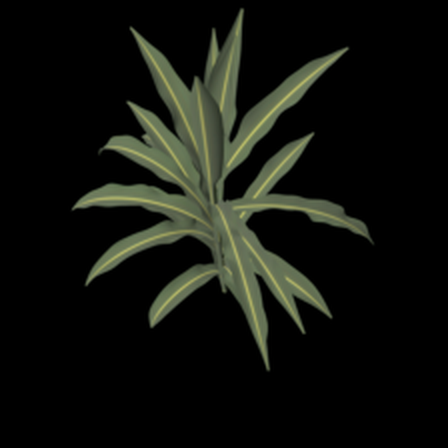
\includegraphics[width=0.4000in, height=0.4000in]{Figures/fig2/image.png}};
\node[anchor=south west, inner sep=0] at (0.9500,3.4600) {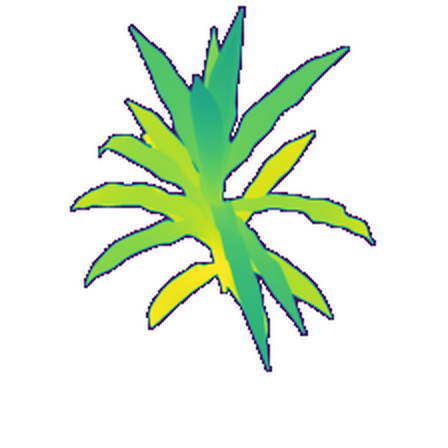
\includegraphics[width=0.4000in, height=0.4000in]{Figures/fig2/depth_image.png}};
\node[anchor=south west, inner sep=0] at (0.5200,3.0300) {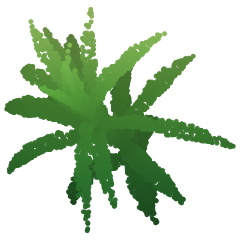
\includegraphics[width=0.4000in, height=0.4000in]{Figures/fig2/point_cloud.png}};
\node[anchor=south west, inner sep=0] at (0.9500,3.0300) {
\includegraphics[width=0.4000in, height=0.4000in]{Figures/fig2/parameters.png}};
\node[anchor=south west, inner sep=0] at (1.5500,3.4600) {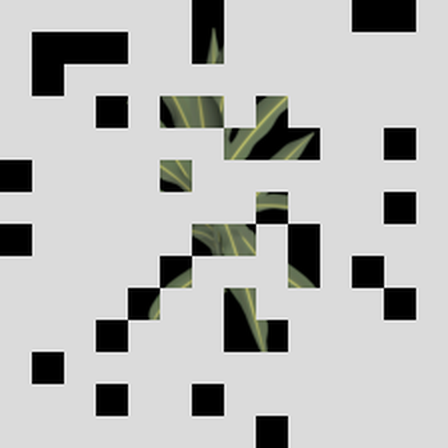
\includegraphics[width=0.4000in, height=0.4000in]{Figures/fig2/image_masked.png}};
\node[anchor=south west, inner sep=0] at (1.9800,3.4600) {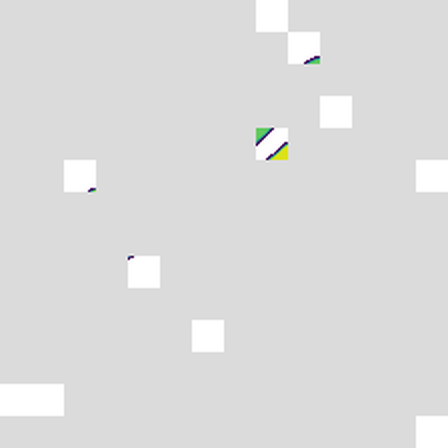
\includegraphics[width=0.4000in, height=0.4000in]{Figures/fig2/depth_masked.png}};
\node[anchor=south west, inner sep=0] at (1.5500,3.0300) {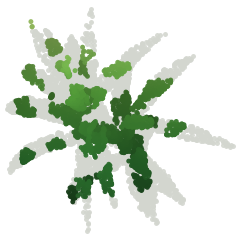
\includegraphics[width=0.4000in, height=0.4000in]{Figures/fig2/cloud_masked.png}};
\node[anchor=south west, inner sep=0] at (1.9800,3.0300) {
\includegraphics[width=0.4000in, height=0.4000in]{Figures/fig2/parameters_masked.png}};
\node[anchor=south west, inner sep=0] at (4.0600,3.4600) {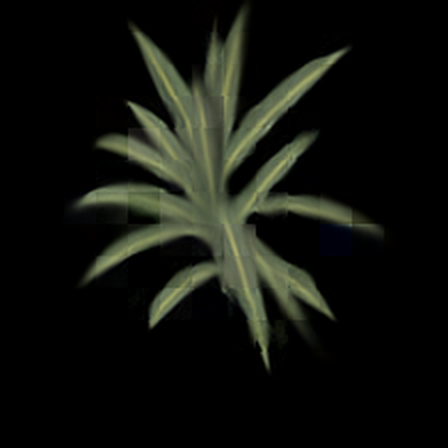
\includegraphics[width=0.4000in, height=0.4000in]{Figures/fig2/image_output.png}};
\node[anchor=south west, inner sep=0] at (4.4900,3.4600) {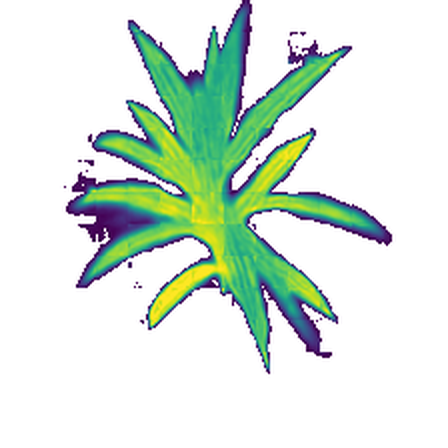
\includegraphics[width=0.4000in, height=0.4000in]{Figures/fig2/depth_output.png}};
\node[anchor=south west, inner sep=0] at (4.0600,3.0300) {
\includegraphics[width=0.4000in, height=0.4000in]{Figures/fig2/cloud_output.png}};
\node[anchor=south west, inner sep=0] at (4.4900,3.0300) {
\includegraphics[width=0.4000in, height=0.4000in]{Figures/fig2/parameters_output.png}};
\node[anchor=south west, inner sep=0] at (3.1950,3.7250) {
\includegraphics[width=0.1700in, height=0.1700in]{Figures/fig2/fire.png}};
\node[anchor=south west, inner sep=0] at (0.5950,2.0250) {
\includegraphics[width=0.1700in, height=0.1700in]{Figures/fig2/snow.png}};
\node[anchor=south west, inner sep=0] at (0.5800,1.6200) {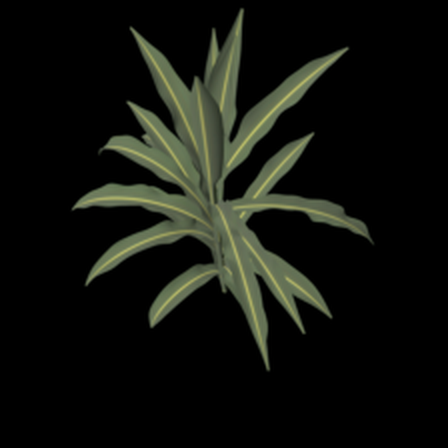
\includegraphics[width=0.2600in, height=0.2600in]{Figures/fig2/teacher_image.png}};
\node[anchor=south west, inner sep=0] at (0.8800,1.6200) {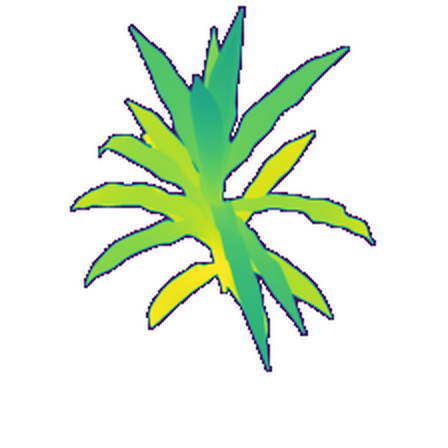
\includegraphics[width=0.2600in, height=0.2600in]{Figures/fig2/teacher_depth_image.png}};
\node[anchor=south west, inner sep=0] at (1.1800,1.6200) {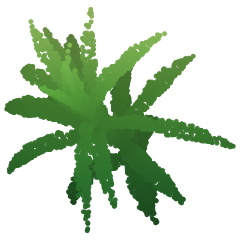
\includegraphics[width=0.2600in, height=0.2600in]{Figures/fig2/teacher_point_cloud.png}};
\node[anchor=south west, inner sep=0] at (1.4800,1.6200) {
\includegraphics[width=0.2600in, height=0.2600in]{Figures/fig2/teacher_parameters.png}};
\node[anchor=south west, inner sep=0] at (2.3750,2.0250) {
\includegraphics[width=0.1700in, height=0.1700in]{Figures/fig2/fire_2.png}};
\node[anchor=south west, inner sep=0] at (2.3600,1.6200) {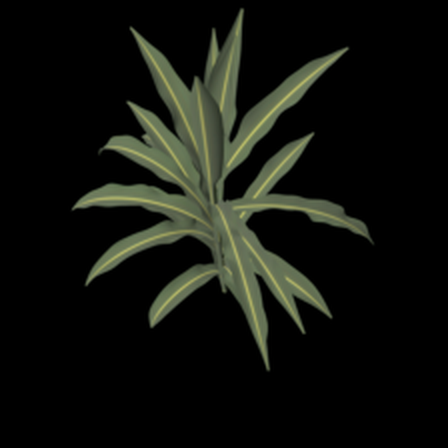
\includegraphics[width=0.2600in, height=0.2600in]{Figures/fig2/student_image.png}};
\node[anchor=south west, inner sep=0] at (2.6600,1.6200) {
\includegraphics[width=0.2600in, height=0.2600in]{Figures/fig2/student_hidden_0.png}};
\node[anchor=south west, inner sep=0] at (2.9600,1.6200) {
\includegraphics[width=0.2600in, height=0.2600in]{Figures/fig2/student_hidden_1.png}};
\node[anchor=south west, inner sep=0] at (3.2600,1.6200) {
\includegraphics[width=0.2600in, height=0.2600in]{Figures/fig2/student_hidden_2.png}};
\node[anchor=south west, inner sep=0] at (3.7500,1.6400) {
\includegraphics[width=0.5800in, height=0.5800in]{Figures/fig2/stage_2_before.png}};
\node[anchor=south west, inner sep=0] at (4.3700,1.6400) {
\includegraphics[width=0.5800in, height=0.5800in]{Figures/fig2/stage_2_after.png}};
\node[anchor=south west, inner sep=0] at (0.5200,0.4400) {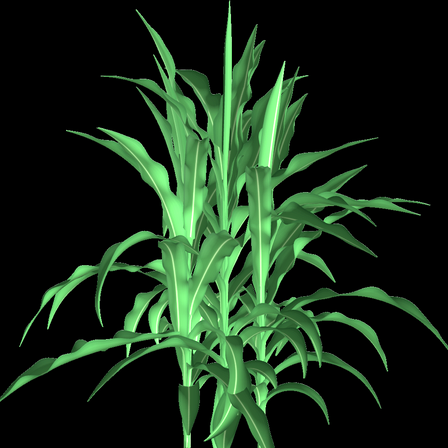
\includegraphics[width=0.4000in, height=0.4000in]{Figures/fig2/row_image.png}};
\node[anchor=south west, inner sep=0] at (0.9600,0.4400) {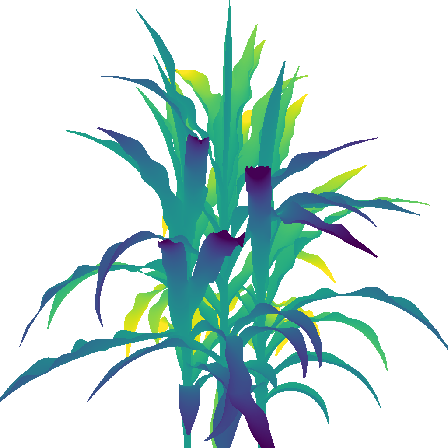
\includegraphics[width=0.4000in, height=0.4000in]{Figures/fig2/row_depth.png}};
\node[anchor=south west, inner sep=0] at (1.4000,0.4400) {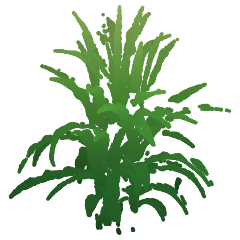
\includegraphics[width=0.4000in, height=0.4000in]{Figures/fig2/row_cloud.png}};
\node[anchor=south west, inner sep=0] at (2.7650,0.7250) {
\includegraphics[width=0.1700in, height=0.1700in]{Figures/fig2/fire_3.png}};
\node[anchor=south west, inner sep=0] at (3.7500,0.3800) {
\includegraphics[width=0.5800in, height=0.5800in]{Figures/fig2/stage_3_before.png}};
\node[anchor=south west, inner sep=0] at (4.3700,0.3800) {
\includegraphics[width=0.5800in, height=0.5800in]{Figures/fig2/stage_3_after.png}};
\node[anchor=west, inner sep=0, outer sep=0, align=left, text=c1D221C, font={\fontsize{9.00}{11.25}\selectfont\sffamily\bfseries}] at (0.6300,4.2800) {Stage 1: masked pretraining};
\node[anchor=west, inner sep=0, outer sep=0, align=left, text=c1D221C, font={\fontsize{9.00}{11.25}\selectfont\sffamily\bfseries}] at (0.6300,2.5600) {Stage 2: cross-modal distillation};
\node[anchor=west, inner sep=0, outer sep=0, align=left, text=c1D221C, font={\fontsize{9.00}{11.25}\selectfont\sffamily\bfseries}] at (0.6300,1.2400) {Stage 3: row fine-tuning};
\draw[draw=cC0392B, line width=1.100pt, -{Triangle[length=2.80pt,width=2.80pt]}] (0.4000,3.4000) .. controls (0.1947,2.9333) and (0.1947,2.4667) .. (0.4000,2.0000);
\draw[draw=cC0392B, line width=1.100pt, -{Triangle[length=2.80pt,width=2.80pt]}] (0.4000,3.2000) .. controls (0.2137,2.3533) and (0.2137,1.5067) .. (0.4000,0.6600);
\node[anchor=center, inner sep=0, outer sep=0, align=center, text=cC0392B, font={\fontsize{9.00}{11.25}\selectfont\sffamily\bfseries}, rotate=90] at (0.1000,2.0000) {warm start};
\draw[draw=cC0392B, line width=0.800pt, rounded corners=0.0300in] (0.5200,3.4600) rectangle (0.9200,3.8600);
\draw[draw=cB8860B, line width=0.800pt, rounded corners=0.0300in] (0.9500,3.4600) rectangle (1.3500,3.8600);
\draw[draw=c2A9D8F, line width=0.800pt, rounded corners=0.0300in] (0.5200,3.0300) rectangle (0.9200,3.4300);
\draw[draw=c30638E, line width=0.800pt, rounded corners=0.0300in] (0.9500,3.0300) rectangle (1.3500,3.4300);
\draw[draw=cC0392B, line width=0.800pt, rounded corners=0.0300in] (1.5500,3.4600) rectangle (1.9500,3.8600);
\draw[draw=cB8860B, line width=0.800pt, rounded corners=0.0300in] (1.9800,3.4600) rectangle (2.3800,3.8600);
\draw[draw=c2A9D8F, line width=0.800pt, rounded corners=0.0300in] (1.5500,3.0300) rectangle (1.9500,3.4300);
\draw[draw=c30638E, line width=0.800pt, rounded corners=0.0300in] (1.9800,3.0300) rectangle (2.3800,3.4300);
\draw[draw=cC0392B, line width=0.800pt, rounded corners=0.0300in] (4.0600,3.4600) rectangle (4.4600,3.8600);
\draw[draw=cB8860B, line width=0.800pt, rounded corners=0.0300in] (4.4900,3.4600) rectangle (4.8900,3.8600);
\draw[draw=c2A9D8F, line width=0.800pt, rounded corners=0.0300in] (4.0600,3.0300) rectangle (4.4600,3.4300);
\draw[draw=c30638E, line width=0.800pt, rounded corners=0.0300in] (4.4900,3.0300) rectangle (4.8900,3.4300);
\node[anchor=south, inner sep=0, outer sep=0, align=center, text=c1D221C, font={\fontsize{9.00}{11.25}\selectfont\sffamily\bfseries}] at (0.9350,3.9600) {Input};
\node[anchor=south, inner sep=0, outer sep=0, align=center, text=c1D221C, font={\fontsize{9.00}{11.25}\selectfont\sffamily\bfseries}] at (1.9650,3.9600) {80 \% hidden};
\node[anchor=south, inner sep=0, outer sep=0, align=center, text=c1D221C, font={\fontsize{9.00}{11.25}\selectfont\sffamily\bfseries}] at (4.4750,3.9600) {Output};
\draw[draw=c1D221C, line width=0.900pt, -{Triangle[length=2.80pt,width=2.80pt]}] (1.3800,3.4450) -- (1.5200,3.4450);
\draw[draw=c1D221C, line width=0.900pt, -{Triangle[length=2.80pt,width=2.80pt]}] (2.4100,3.4450) -- (2.5900,3.4450);
\node[anchor=center, inner sep=0, outer sep=0, align=center, text=c2B3A67, font={\fontsize{9.00}{11.25}\selectfont\sffamily\bfseries}] at (2.9293,3.4450) {Encoder};
\node[anchor=center, inner sep=0, outer sep=0, align=center, text=c2B3A67, font={\fontsize{9.00}{11.25}\selectfont\sffamily\bfseries}] at (3.6137,3.4450) {Decoder};
\draw[draw=c1D221C, line width=0.900pt, -{Triangle[length=2.80pt,width=2.80pt]}] (3.9300,3.4450) -- (4.0300,3.4450);
\draw[draw=cC0392B, line width=0.900pt, -{Triangle[length=2.80pt,width=2.80pt]}, dash pattern=on 2.70pt off 1.80pt] (4.4750,2.9500) -- (0.9350,2.9500);
\node[anchor=north, inner sep=0, outer sep=0, align=center, text=cC0392B, font={\fontsize{9.00}{11.25}\selectfont\sffamily}] at (2.6900,2.9000) {loss on the hidden tokens};
\node[anchor=west, inner sep=0, outer sep=0, align=left, text=c1D221C, font={\fontsize{9.00}{11.25}\selectfont\sffamily\bfseries}] at (0.8000,2.1100) {Teacher};
\draw[draw=cC0392B, line width=0.600pt, rounded corners=0.0300in] (0.5800,1.6200) rectangle (0.8400,1.8800);
\draw[draw=cB8860B, line width=0.600pt, rounded corners=0.0300in] (0.8800,1.6200) rectangle (1.1400,1.8800);
\draw[draw=c2A9D8F, line width=0.600pt, rounded corners=0.0300in] (1.1800,1.6200) rectangle (1.4400,1.8800);
\draw[draw=c30638E, line width=0.600pt, rounded corners=0.0300in] (1.4800,1.6200) rectangle (1.7400,1.8800);
\draw[draw=cC0392B, line width=0.900pt, -{Triangle[length=2.80pt,width=2.80pt]}, dash pattern=on 2.70pt off 1.80pt] (1.8000,1.8800) -- (2.2700,1.8800);
\node[anchor=south, inner sep=0, outer sep=0, align=center, text=cC0392B, font={\fontsize{9.00}{11.25}\selectfont\sffamily}] at (2.0350,1.9300) {features};
\node[anchor=west, inner sep=0, outer sep=0, align=left, text=c2B3A67, font={\fontsize{9.00}{11.25}\selectfont\sffamily\bfseries}] at (2.5800,2.1100) {Student};
\draw[draw=cC0392B, line width=0.900pt, rounded corners=0.0300in] (2.3600,1.6200) rectangle (2.6200,1.8800);
\draw[draw=cB8860B, line width=0.600pt, dash pattern=on 1.80pt off 1.20pt, rounded corners=0.0300in] (2.6600,1.6200) rectangle (2.9200,1.8800);
\draw[draw=c2A9D8F, line width=0.600pt, dash pattern=on 1.80pt off 1.20pt, rounded corners=0.0300in] (2.9600,1.6200) rectangle (3.2200,1.8800);
\draw[draw=c30638E, line width=0.600pt, dash pattern=on 1.80pt off 1.20pt, rounded corners=0.0300in] (3.2600,1.6200) rectangle (3.5200,1.8800);
\draw[draw=c1D221C, line width=0.900pt, -{Triangle[length=2.80pt,width=2.80pt]}] (3.5800,1.9100) -- (3.7200,1.9100);
\draw[draw=c5F685C, line width=0.800pt, dash pattern=on 2.40pt off 1.60pt, rounded corners=0.0300in] (3.7500,1.6400) rectangle (4.3300,2.2200);
\node[anchor=south, inner sep=0, outer sep=0, align=center, text=c5F685C, font={\fontsize{9.00}{11.25}\selectfont\sffamily}] at (4.0400,2.2700) {before};
\draw[draw=c2A9D8F, line width=0.800pt, rounded corners=0.0300in] (4.3700,1.6400) rectangle (4.9500,2.2200);
\node[anchor=south, inner sep=0, outer sep=0, align=center, text=c2B3A67, font={\fontsize{9.00}{11.25}\selectfont\sffamily\bfseries}] at (4.6600,2.2700) {after};
\node[anchor=north, inner sep=0, outer sep=0, align=center, text=c1D221C, font={\fontsize{9.00}{11.25}\selectfont\sffamily}] at (4.3500,1.5800) {Chamfer 2.27 $\rightarrow$ 0.88};
\draw[draw=cC0392B, line width=0.800pt, rounded corners=0.0300in] (0.5200,0.4400) rectangle (0.9200,0.8400);
\draw[draw=cB8860B, line width=0.800pt, rounded corners=0.0300in] (0.9600,0.4400) rectangle (1.3600,0.8400);
\draw[draw=c2A9D8F, line width=0.800pt, rounded corners=0.0300in] (1.4000,0.4400) rectangle (1.8000,0.8400);
\node[anchor=south, inner sep=0, outer sep=0, align=center, text=c1D221C, font={\fontsize{9.00}{11.25}\selectfont\sffamily\bfseries}] at (1.1600,0.9200) {Crop row};
\draw[draw=c1D221C, line width=0.900pt, -{Triangle[length=2.80pt,width=2.80pt]}] (1.8500,0.6400) -- (2.2000,0.6400);
\node[anchor=center, inner sep=0, outer sep=0, align=center, text=c2B3A67, font={\fontsize{9.00}{11.25}\selectfont\sffamily\bfseries}] at (2.5194,0.6400) {Enc};
\node[anchor=center, inner sep=0, outer sep=0, align=center, text=c2B3A67, font={\fontsize{9.00}{11.25}\selectfont\sffamily\bfseries}] at (3.1621,0.6400) {Dec};
\node[anchor=north, inner sep=0, outer sep=0, align=center, text=cC0392B, font={\fontsize{9.00}{11.25}\selectfont\sffamily}] at (2.8300,0.3500) {loss: center plant only};
\draw[draw=c1D221C, line width=0.900pt, -{Triangle[length=2.80pt,width=2.80pt]}] (3.4600,0.6400) -- (3.7200,0.6400);
\draw[draw=c5F685C, line width=0.800pt, dash pattern=on 2.40pt off 1.60pt, rounded corners=0.0300in] (3.7500,0.3800) rectangle (4.3300,0.9600);
\node[anchor=south, inner sep=0, outer sep=0, align=center, text=c5F685C, font={\fontsize{9.00}{11.25}\selectfont\sffamily}] at (4.0400,1.0100) {before};
\draw[draw=c2A9D8F, line width=0.800pt, rounded corners=0.0300in] (4.3700,0.3800) rectangle (4.9500,0.9600);
\node[anchor=south, inner sep=0, outer sep=0, align=center, text=c2B3A67, font={\fontsize{9.00}{11.25}\selectfont\sffamily\bfseries}] at (4.6600,1.0100) {after};
\node[anchor=north, inner sep=0, outer sep=0, align=center, text=c1D221C, font={\fontsize{9.00}{11.25}\selectfont\sffamily}] at (4.3500,0.3200) {Chamfer 230 $\rightarrow$ 31};
\node[anchor=center, inner sep=0, outer sep=0, align=center, text=c1D221C, font={\fontsize{9.00}{11.25}\selectfont\sffamily\bfseries}] at (5.9775,4.0600) {Inside CropCode};
\node[anchor=west, inner sep=0, outer sep=0, align=left, text=cC0392B, font={\fontsize{9.00}{11.25}\selectfont\sffamily\bfseries}] at (5.9250,3.7100) {Image  196};
\node[anchor=west, inner sep=0, outer sep=0, align=left, text=cB8860B, font={\fontsize{9.00}{11.25}\selectfont\sffamily\bfseries}] at (5.9250,3.4100) {Depth  196};
\node[anchor=west, inner sep=0, outer sep=0, align=left, text=c2A9D8F, font={\fontsize{9.00}{11.25}\selectfont\sffamily\bfseries}] at (5.9250,3.1100) {Cloud  196};
\node[anchor=west, inner sep=0, outer sep=0, align=left, text=c30638E, font={\fontsize{9.00}{11.25}\selectfont\sffamily\bfseries}] at (5.9250,2.8100) {Params  1+K};
\node[anchor=west, inner sep=0, outer sep=0, align=left, text=c5F685C, font={\fontsize{9.00}{11.25}\selectfont\sffamily}] at (5.2400,2.5200) {tokens (hollow = hidden)};
\node[anchor=west, inner sep=0, outer sep=0, align=left, text=c1D221C, font={\fontsize{9.00}{11.25}\selectfont\sffamily\bfseries}] at (5.2400,2.2000) {Dirichlet split};
\node[anchor=west, inner sep=0, outer sep=0, align=left, text=c5F685C, font={\fontsize{9.00}{11.25}\selectfont\sffamily}] at (5.2400,1.7600) {of the visible tokens};
\node[anchor=center, inner sep=0, outer sep=0, align=center, text=c2B3A67, font={\fontsize{9.00}{11.25}\selectfont\sffamily\bfseries}] at (5.9775,1.2700) {Encoder, 12 blocks};
\node[anchor=center, inner sep=0, outer sep=0, align=center, text=c2B3A67, font={\fontsize{9.00}{11.25}\selectfont\sffamily\bfseries}] at (5.9775,0.7100) {Decoder, 8 blocks};
\draw[draw=c2B3A67, line width=0.800pt, -{Triangle[length=2.80pt,width=2.80pt]}] (5.9775,1.6200) -- (5.9775,1.4900);
\draw[draw=c2B3A67, line width=0.800pt, -{Triangle[length=2.80pt,width=2.80pt]}] (5.9775,1.0500) -- (5.9775,0.9300);
\draw[draw=c2B3A67, line width=0.800pt, -{Triangle[length=2.80pt,width=2.80pt]}] (5.9775,0.4900) -- (5.9775,0.4200);
\node[anchor=center, inner sep=0, outer sep=0, align=center, text=c2B3A67, font={\fontsize{9.00}{11.25}\selectfont\sffamily}] at (5.9775,0.3200) {one head per stream};
\end{tikzpicture}%
}%
